\documentclass[14pt]{extbook}
\usepackage{multicol, enumerate, enumitem, hyperref, color, soul, setspace, parskip, fancyhdr} %General Packages
\usepackage{amssymb, amsthm, amsmath, bbm, latexsym, units, mathtools} %Math Packages
\everymath{\displaystyle} %All math in Display Style
% Packages with additional options
\usepackage[headsep=0.5cm,headheight=12pt, left=1 in,right= 1 in,top= 1 in,bottom= 1 in]{geometry}
\usepackage[usenames,dvipsnames]{xcolor}
\usepackage{dashrule}  % Package to use the command below to create lines between items
\newcommand{\litem}[1]{\item#1\hspace*{-1cm}\rule{\textwidth}{0.4pt}}
\pagestyle{fancy}
\lhead{Progress Quiz 2}
\chead{}
\rhead{Version C}
\lfoot{7862-5421}
\cfoot{}
\rfoot{Spring 2021}
\begin{document}

\begin{enumerate}
\litem{
Solve the quadratic equation below. Then, choose the intervals that the solutions $x_1$ and $x_2$ belong to, with $x_1 \leq x_2$.\[ 25x^{2} -60 x + 36 = 0 \]\begin{enumerate}[label=\Alph*.]
\item \( x_1 \in [0.27, 0.47] \text{ and } x_2 \in [2.55, 4.19] \)
\item \( x_1 \in [0.22, 0.28] \text{ and } x_2 \in [4.87, 6.93] \)
\item \( x_1 \in [0.51, 0.69] \text{ and } x_2 \in [2.04, 2.84] \)
\item \( x_1 \in [1.02, 1.23] \text{ and } x_2 \in [0.71, 1.59] \)
\item \( x_1 \in [29.96, 30.12] \text{ and } x_2 \in [29.98, 31.87] \)

\end{enumerate} }
\litem{
Solve the quadratic equation below. Then, choose the intervals that the solutions $x_1$ and $x_2$ belong to, with $x_1 \leq x_2$.\[ 25x^{2} -50 x + 24 = 0 \]\begin{enumerate}[label=\Alph*.]
\item \( x_1 \in [0.66, 1.05] \text{ and } x_2 \in [1.03, 1.54] \)
\item \( x_1 \in [19.99, 20.16] \text{ and } x_2 \in [29.03, 30.63] \)
\item \( x_1 \in [0.52, 0.67] \text{ and } x_2 \in [1.21, 1.76] \)
\item \( x_1 \in [0.21, 0.36] \text{ and } x_2 \in [3.46, 4.01] \)
\item \( x_1 \in [0.35, 0.43] \text{ and } x_2 \in [2.13, 2.95] \)

\end{enumerate} }
\litem{
Write the equation of the graph presented below in the form $f(x)=ax^2+bx+c$, assuming  $a=1$ or $a=-1$. Then, choose the intervals that $a, b,$ and $c$ belong to.
\begin{center}
    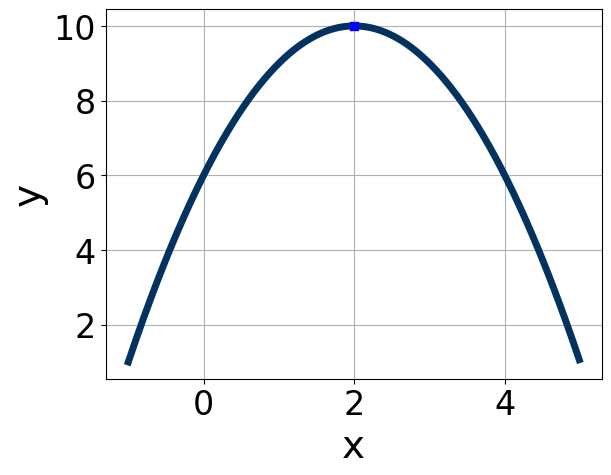
\includegraphics[width=0.5\textwidth]{../Figures/quadraticGraphToEquationCopyC.png}
\end{center}
\begin{enumerate}[label=\Alph*.]
\item \( a \in [-4, 0], \hspace*{5mm} b \in [-7, 2], \text{ and } \hspace*{5mm} c \in [-16, -12] \)
\item \( a \in [1, 2], \hspace*{5mm} b \in [-7, 2], \text{ and } \hspace*{5mm} c \in [14, 19] \)
\item \( a \in [-4, 0], \hspace*{5mm} b \in [2, 6], \text{ and } \hspace*{5mm} c \in [4, 8] \)
\item \( a \in [1, 2], \hspace*{5mm} b \in [2, 6], \text{ and } \hspace*{5mm} c \in [14, 19] \)
\item \( a \in [-4, 0], \hspace*{5mm} b \in [-7, 2], \text{ and } \hspace*{5mm} c \in [4, 8] \)

\end{enumerate} }
\litem{
Solve the quadratic equation below. Then, choose the intervals that the solutions belong to, with $x_1 \leq x_2$ (if they exist).\[ 14x^{2} -12 x -9 = 0 \]\begin{enumerate}[label=\Alph*.]
\item \( x_1 \in [-7.04, -6.25] \text{ and } x_2 \in [18.1, 20.5] \)
\item \( x_1 \in [-0.85, -0.32] \text{ and } x_2 \in [0.7, 2.2] \)
\item \( x_1 \in [-1.78, -1.31] \text{ and } x_2 \in [-0.5, 1] \)
\item \( x_1 \in [-25.55, -24.82] \text{ and } x_2 \in [24.9, 26.1] \)
\item \( \text{There are no Real solutions.} \)

\end{enumerate} }
\litem{
Write the equation of the graph presented below in the form $f(x)=ax^2+bx+c$, assuming  $a=1$ or $a=-1$. Then, choose the intervals that $a, b,$ and $c$ belong to.
\begin{center}
    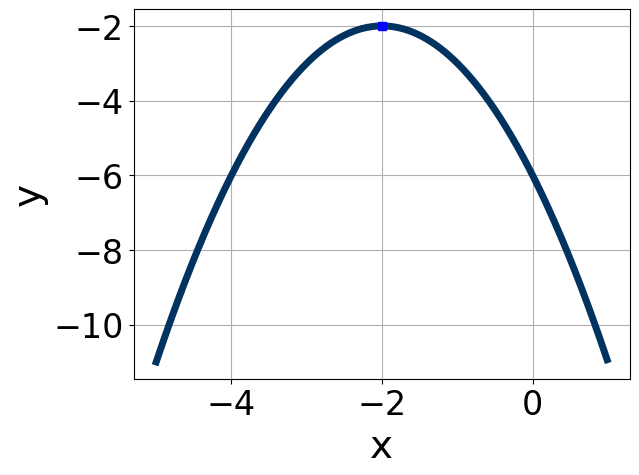
\includegraphics[width=0.5\textwidth]{../Figures/quadraticGraphToEquationC.png}
\end{center}
\begin{enumerate}[label=\Alph*.]
\item \( a \in [-2.2, 0.2], \hspace*{5mm} b \in [2, 6], \text{ and } \hspace*{5mm} c \in [-6, -4] \)
\item \( a \in [-2.2, 0.2], \hspace*{5mm} b \in [2, 6], \text{ and } \hspace*{5mm} c \in [-4, -1] \)
\item \( a \in [0.6, 3], \hspace*{5mm} b \in [2, 6], \text{ and } \hspace*{5mm} c \in [0, 3] \)
\item \( a \in [-2.2, 0.2], \hspace*{5mm} b \in [-6, -2], \text{ and } \hspace*{5mm} c \in [-6, -4] \)
\item \( a \in [0.6, 3], \hspace*{5mm} b \in [-6, -2], \text{ and } \hspace*{5mm} c \in [0, 3] \)

\end{enumerate} }
\litem{
Graph the equation below.\[ f(x) = (x-4)^2 + 20 \]\begin{enumerate}[label=\Alph*.]
\begin{multicols}{2}\item 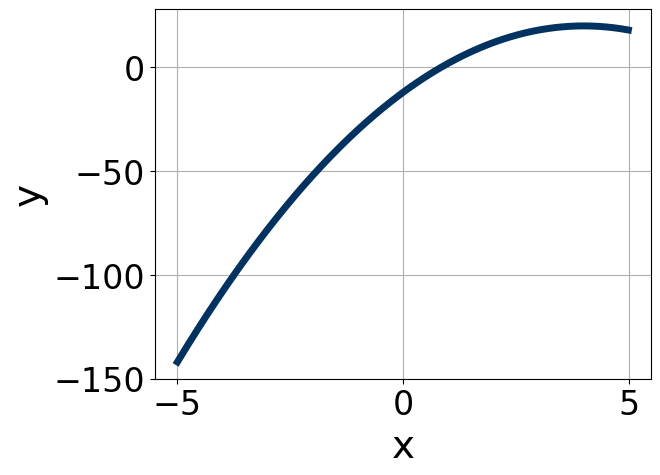
\includegraphics[width = 0.3\textwidth]{../Figures/quadraticEquationToGraphCopyAC.png}\item 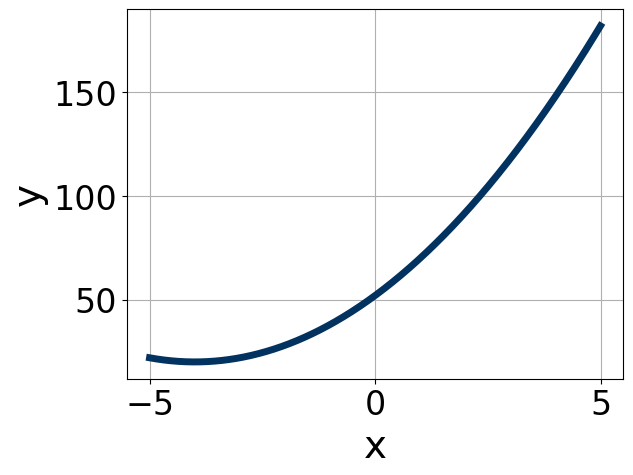
\includegraphics[width = 0.3\textwidth]{../Figures/quadraticEquationToGraphCopyBC.png}\item 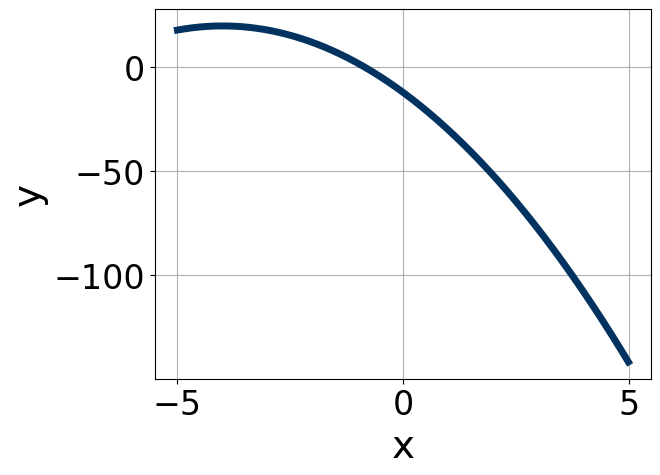
\includegraphics[width = 0.3\textwidth]{../Figures/quadraticEquationToGraphCopyCC.png}\item 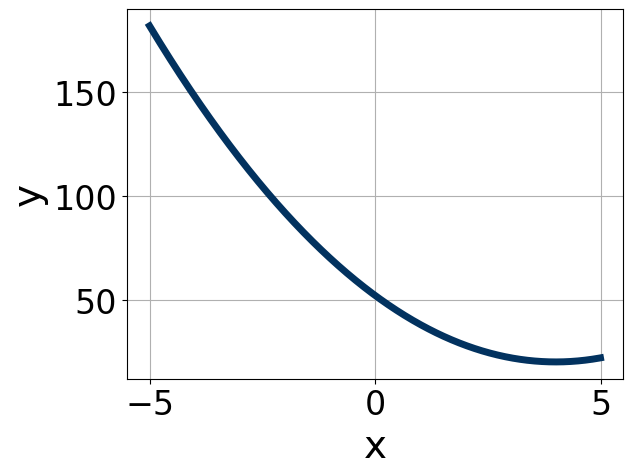
\includegraphics[width = 0.3\textwidth]{../Figures/quadraticEquationToGraphCopyDC.png}\end{multicols}\item None of the above.
\end{enumerate} }
\litem{
Graph the equation below.\[ f(x) = (x-2)^2 - 18 \]\begin{enumerate}[label=\Alph*.]
\begin{multicols}{2}\item 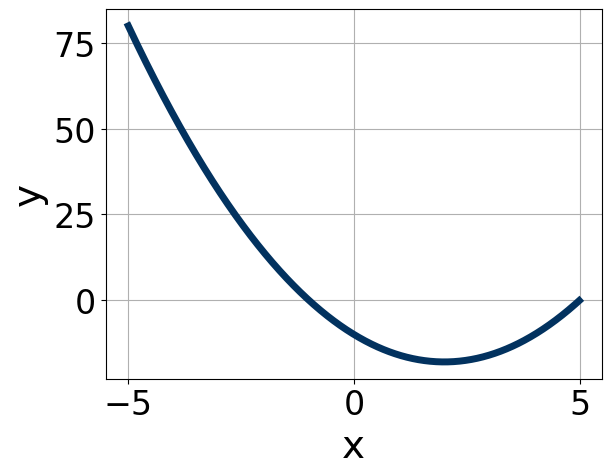
\includegraphics[width = 0.3\textwidth]{../Figures/quadraticEquationToGraphAC.png}\item 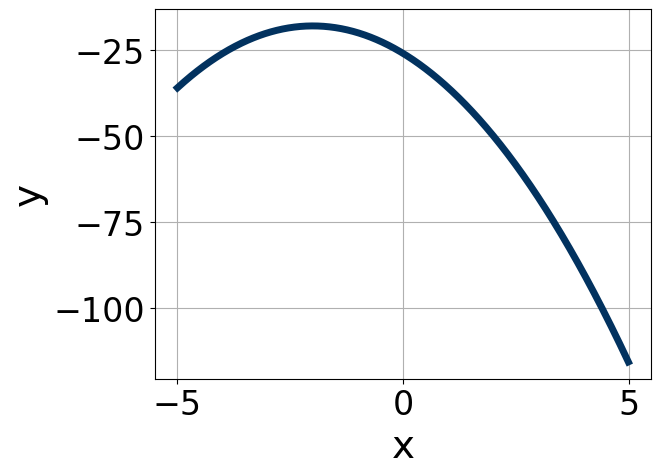
\includegraphics[width = 0.3\textwidth]{../Figures/quadraticEquationToGraphBC.png}\item 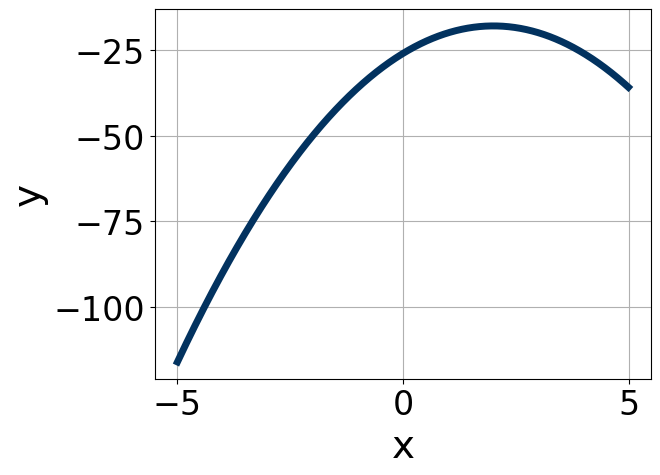
\includegraphics[width = 0.3\textwidth]{../Figures/quadraticEquationToGraphCC.png}\item 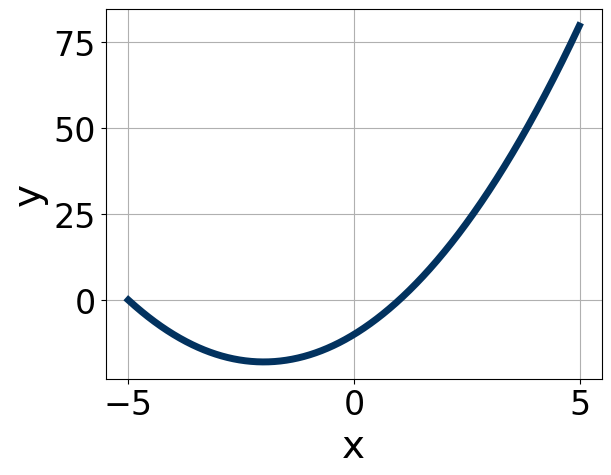
\includegraphics[width = 0.3\textwidth]{../Figures/quadraticEquationToGraphDC.png}\end{multicols}\item None of the above.
\end{enumerate} }
\litem{
Factor the quadratic below. Then, choose the intervals that contain the constants in the form $(ax+b)(cx+d); b \leq d.$\[ 36x^{2} +60 x + 25 \]\begin{enumerate}[label=\Alph*.]
\item \( a \in [0.83, 2.1], \hspace*{5mm} b \in [26, 36], \hspace*{5mm} c \in [0.31, 1.2], \text{ and } \hspace*{5mm} d \in [26, 33] \)
\item \( a \in [17.63, 18.91], \hspace*{5mm} b \in [4, 9], \hspace*{5mm} c \in [1.89, 2.19], \text{ and } \hspace*{5mm} d \in [2, 8] \)
\item \( a \in [5.82, 6.65], \hspace*{5mm} b \in [4, 9], \hspace*{5mm} c \in [5.79, 7.41], \text{ and } \hspace*{5mm} d \in [2, 8] \)
\item \( a \in [1.3, 3.45], \hspace*{5mm} b \in [4, 9], \hspace*{5mm} c \in [10.82, 13.06], \text{ and } \hspace*{5mm} d \in [2, 8] \)
\item \( \text{None of the above.} \)

\end{enumerate} }
\litem{
Solve the quadratic equation below. Then, choose the intervals that the solutions belong to, with $x_1 \leq x_2$ (if they exist).\[ 19x^{2} -11 x -2 = 0 \]\begin{enumerate}[label=\Alph*.]
\item \( x_1 \in [-2.86, -2.46] \text{ and } x_2 \in [13.6, 14.1] \)
\item \( x_1 \in [-0.92, -0.57] \text{ and } x_2 \in [-1.9, 0.4] \)
\item \( x_1 \in [-16.39, -16.21] \text{ and } x_2 \in [15.8, 18.4] \)
\item \( x_1 \in [-0.2, 0.03] \text{ and } x_2 \in [0.6, 2.8] \)
\item \( \text{There are no Real solutions.} \)

\end{enumerate} }
\litem{
Factor the quadratic below. Then, choose the intervals that contain the constants in the form $(ax+b)(cx+d); b \leq d.$\[ 24x^{2} -38 x + 15 \]\begin{enumerate}[label=\Alph*.]
\item \( a \in [1.8, 4.4], \hspace*{5mm} b \in [-6, -4], \hspace*{5mm} c \in [6.95, 9.24], \text{ and } \hspace*{5mm} d \in [-3, -1] \)
\item \( a \in [4, 7.9], \hspace*{5mm} b \in [-6, -4], \hspace*{5mm} c \in [3.87, 4.05], \text{ and } \hspace*{5mm} d \in [-3, -1] \)
\item \( a \in [10.9, 13.8], \hspace*{5mm} b \in [-6, -4], \hspace*{5mm} c \in [1.9, 2.61], \text{ and } \hspace*{5mm} d \in [-3, -1] \)
\item \( a \in [0.8, 1.2], \hspace*{5mm} b \in [-22, -16], \hspace*{5mm} c \in [0.75, 1.4], \text{ and } \hspace*{5mm} d \in [-23, -13] \)
\item \( \text{None of the above.} \)

\end{enumerate} }
\end{enumerate}

\end{document}